\newpage
\chapter{Funktionen}
In der realen Welt begegnen uns h"aufig Abh"angigkeiten zwischen
zwei Gr"o"sen.\\
Als Beispiel hierf"ur sei die Fl"ache einer geometrischen Grundk"orpers
ist abh"angig von der Seitenl"ange eines Quadrats, oder bei einen Kreis,
dessen Radius. \\
Um die Abh"angigkeiten besser verstehen zu k"onnen, spricht man auch von
einer Zuordnung eines Wertes zu einen anderen Wert.\\
\\
Beispiel:\\
Der Hefeteig eines Kuchens hat in der ersten Stunde das doppelte Volumen.
In der zweiten Stunde hat der Teig das doppelte Volumen des Vorg"angers. \\
\\
Erst wenn wir verstanden haben, was eine Zuordnung ist, k"onnen wir uns
mit Funktionen n"aher besch"aftigen. Grund daf"ur ist, dass eine Funktion
nichts anderes als eine Zuordnung mit bestimmten Eigenschaften ist.\\
Außerdem m"ussen wir unseren mathematischen Wortschatz um einige Vokabeln
erweitern.
\\
\begin{tabular}{p{4cm}p{7cm}}
  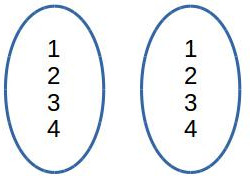
\includegraphics[width=0.3\textwidth]{pics/menge1.jpg} &
  \vtop{\vskip -64pt \vskip -\ht\strutbox 
    \begin{tabular}{lp{4cm}}
      Die linke Mengen wird als Definitions(menge) \\
      bezeichnet, w"ahrend die rechte Menge als \\
      Werte(menge) bezeichnet wird.
    \end{tabular}\vskip -\dp\strutbox }%
\end{tabular}
\\
\begin{tabular}{p{4cm}p{7cm}}
  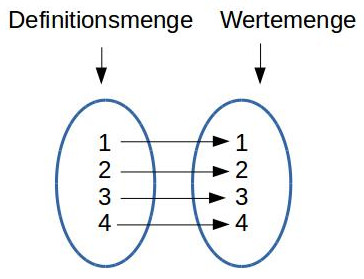
\includegraphics[width=0.3\textwidth]{pics/menge3.jpg} &
  \vtop{\vskip -64pt \vskip -\ht\strutbox 
    \begin{tabular}{lp{4cm}}
      Wie wir bereits wissen, besteht zwischen den \\
      beiden Mengen eine Beziehung. Diese Beziehung \\
      l"asst sich mit Zuordnungspfeilen verdeutlichen. \\
      \\
      $ 1 \mapsto 1 $ \\
      $ \ldots $ \\
      $ 4 \mapsto 4 $
    \end{tabular}\vskip -\dp\strutbox }%
\end{tabular}
\\
\begin{tabular}{p{4cm}p{7cm}}
  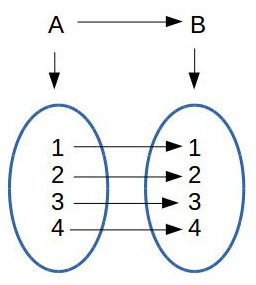
\includegraphics[width=0.3\textwidth]{pics/menge4.jpg} &
  \vtop{\vskip -64pt \vskip -\ht\strutbox 
    \begin{tabular}{lp{4cm}}
      Bei $ f: A \mapsto B $ handelt es sich um eine Funktion, \\
      da jedem Element x der Menge A genau ein Element \\
      y der  Menge B zugeordnet ist. 
    \end{tabular}\vskip -\dp\strutbox }%
\end{tabular}
\\
\begin{tabular}{p{4cm}p{7cm}}
  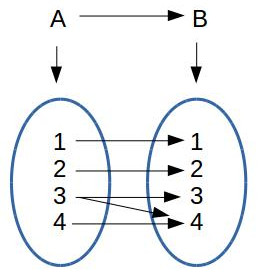
\includegraphics[width=0.3\textwidth]{pics/menge5.jpg} &
  \vtop{\vskip -64pt \vskip -\ht\strutbox 
    \begin{tabular}{lp{4cm}}
      Bei $ f: A \mapsto B $ handelt es sich um keine Funktion, \\
      da dem Element 3 der Menge A zwei Elemente \\
      (3 und 4) der Menge B zugeordnet sind. 4
    \end{tabular}\vskip -\dp\strutbox }%
\end{tabular}
\\
\begin{tabular}{p{4cm}p{7cm}}
  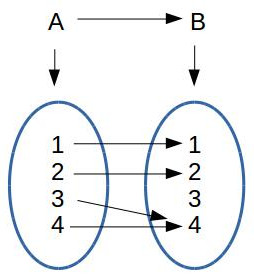
\includegraphics[width=0.3\textwidth]{pics/menge6.jpg} &
  \vtop{\vskip -79pt \vskip -\ht\strutbox 
    \begin{tabular}{lp{4cm}}
    Bei $ f: A \mapsto B $ handelt es sich um eine Funktion, \\
    da jedem Element x der Menge A genau ein Element y der \\
    Menge B zugeordnet ist. \\
    \\
    Dass sich einem Element aus der Menge B zwei Elemente \\
    der Menge A zuordnen lassen, spielt keine Rolle. \\
    Es handelt sich laut Definition trotzdem um eine Funktion.
    \end{tabular}\vskip -\dp\strutbox }%
\end{tabular}
\\
Die Erkenntnisse aus den obigen Beispielen lassen sich folgendermaßen zusammenfassen:
Eine Funktion liegt vor, wenn von jedem Element x der linken Menge (Definitionsmenge)
genau ein Pfeil abgeht.
Von wie vielen Pfeilen ein Element y der rechten Menge (Wertemenge)
getroffen wird, spielt dagegen f"ur die Definition einer Funktion keine Rolle. \\
\\
\textbf{Bezeichnungen und Schreibweisen}
\\
Leider verwenden nicht alle Autoren/Lehrer dieselben Begriffe.
Es ist deshalb notwendig, dass man die alternativen Bezeichnungen
im Hinterkopf beh"alt, um Verwirrungen beim Lesen verschiedener Mathematiktexte
zu vermeiden. \\
\\
Zwei Funktionen sind genau dann identisch, wenn sie in folgenden Teilen "ubereinstimmen:\\
\\
* Funktionsgleichung \\
* Definitionsmenge \\
* Wertemenge \\
\\
Demzufolge sind zwei Funktionen mit gleicher Funktionsgleichung, aber verschiedenen Definitionsmengen
oder verschiedenen Wertemengen, nicht identisch und k"onnen somit unterschiedliche Eigenschaften besitzen. \\
\\
\textbf{Beispiele einer Funktion:} \\
$ y = 2x , \: D = \{ 1, 2, 3 \} , \: W = \{ 2, 4, 8 \} $ \\

